\section{Exclusion Range Comparison Study}
\label{sec:ExclusionRangeStudy}

We verify that the fit is not sensitive to the exclusion window by varying the exclusion
range within $\pm 10~{\mbox{GeV}}$. Specifically, we move the lower boundary of the
window from $120$ to $140$ in increments of $2~{\mbox{GeV}}$ (the width of the window is
 $42~{\mbox{GeV}}$). The results are shown in Fig.~\ref{fig:ExclusionRangeScan}.
The fluctuations in the total yield are within the corresponding uncertainties and we
conclude that the fit is stable.

%%%%%%%
\begin{figure}[h!] {\centering
\unitlength=0.33\linewidth
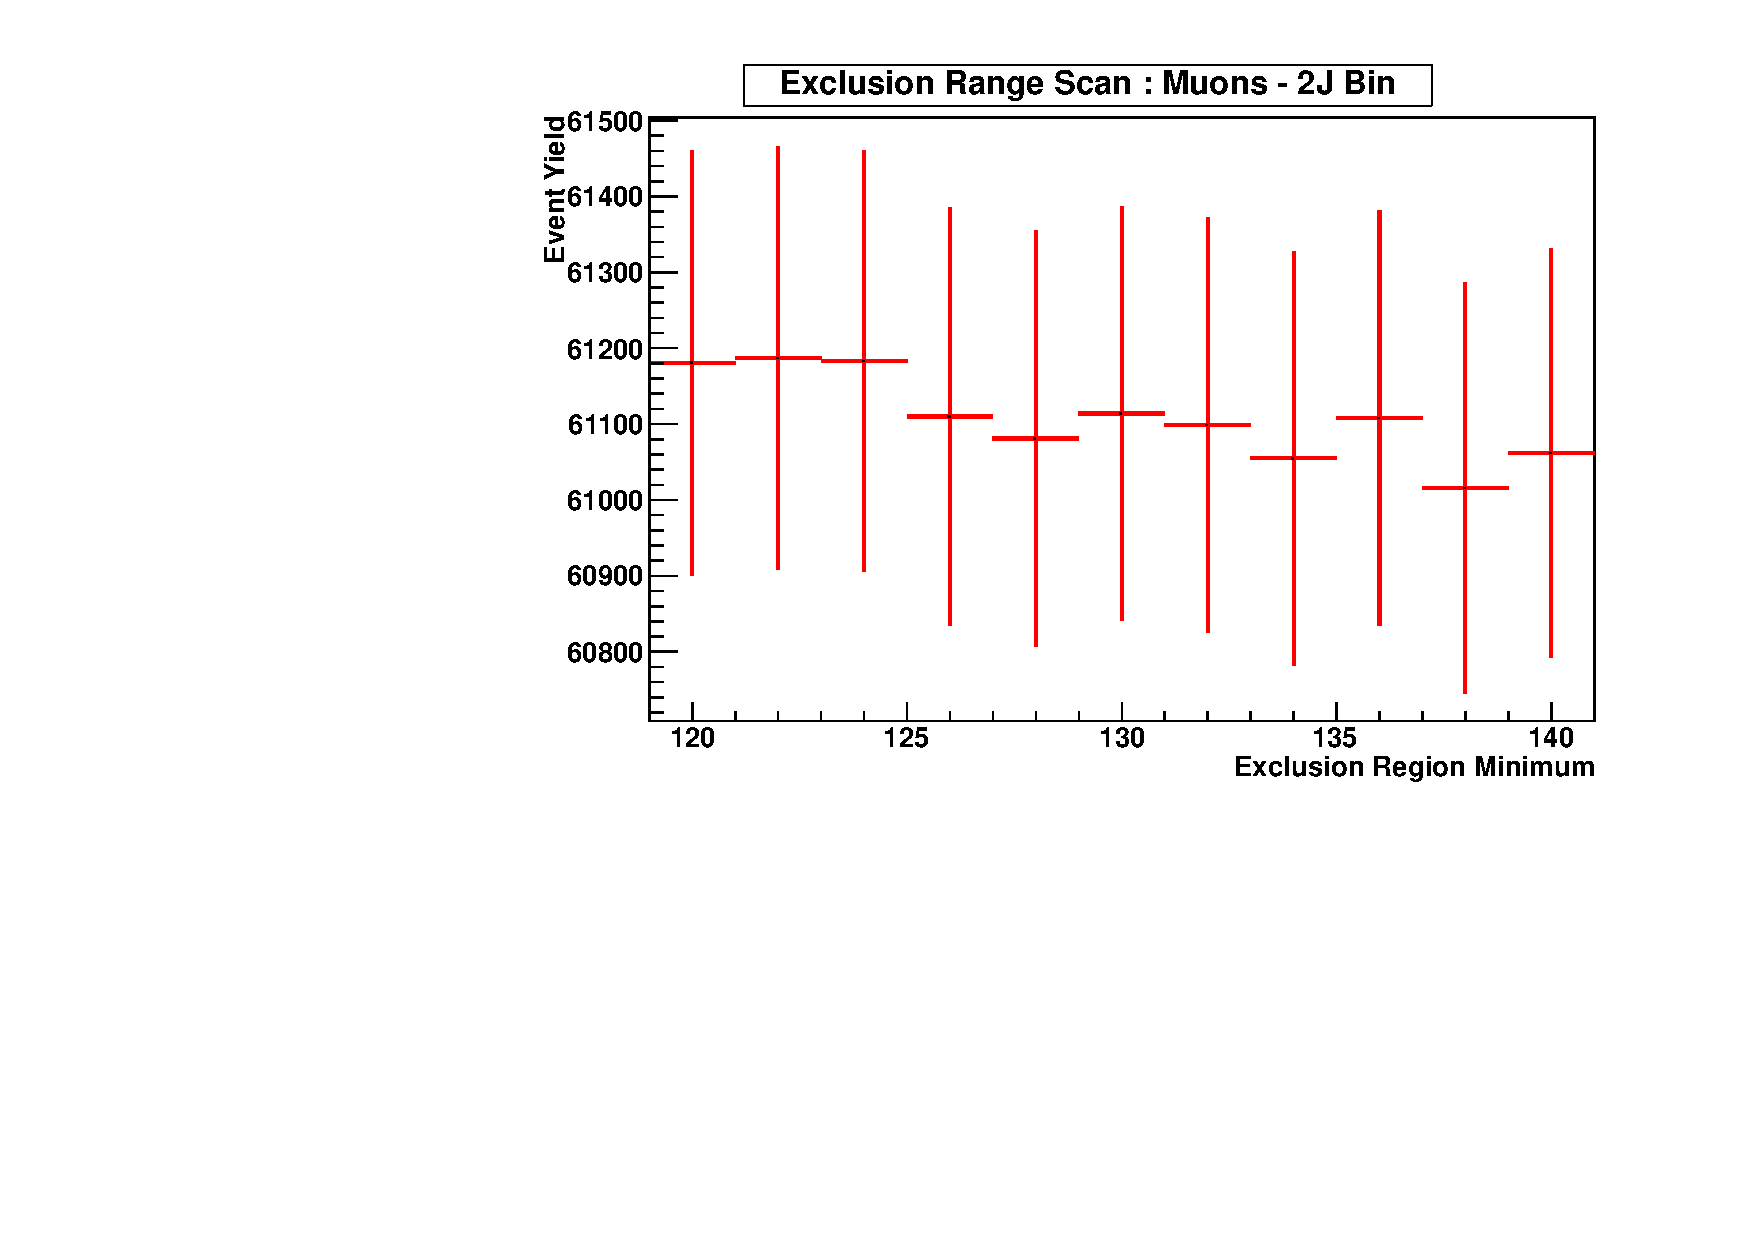
\includegraphics[width=0.48\textwidth]{figs/AdditionalStudies/ExclusionRangeScan_mu2J.pdf}
\put(-0.80,0.0){(a)} 
\unitlength=0.33\linewidth
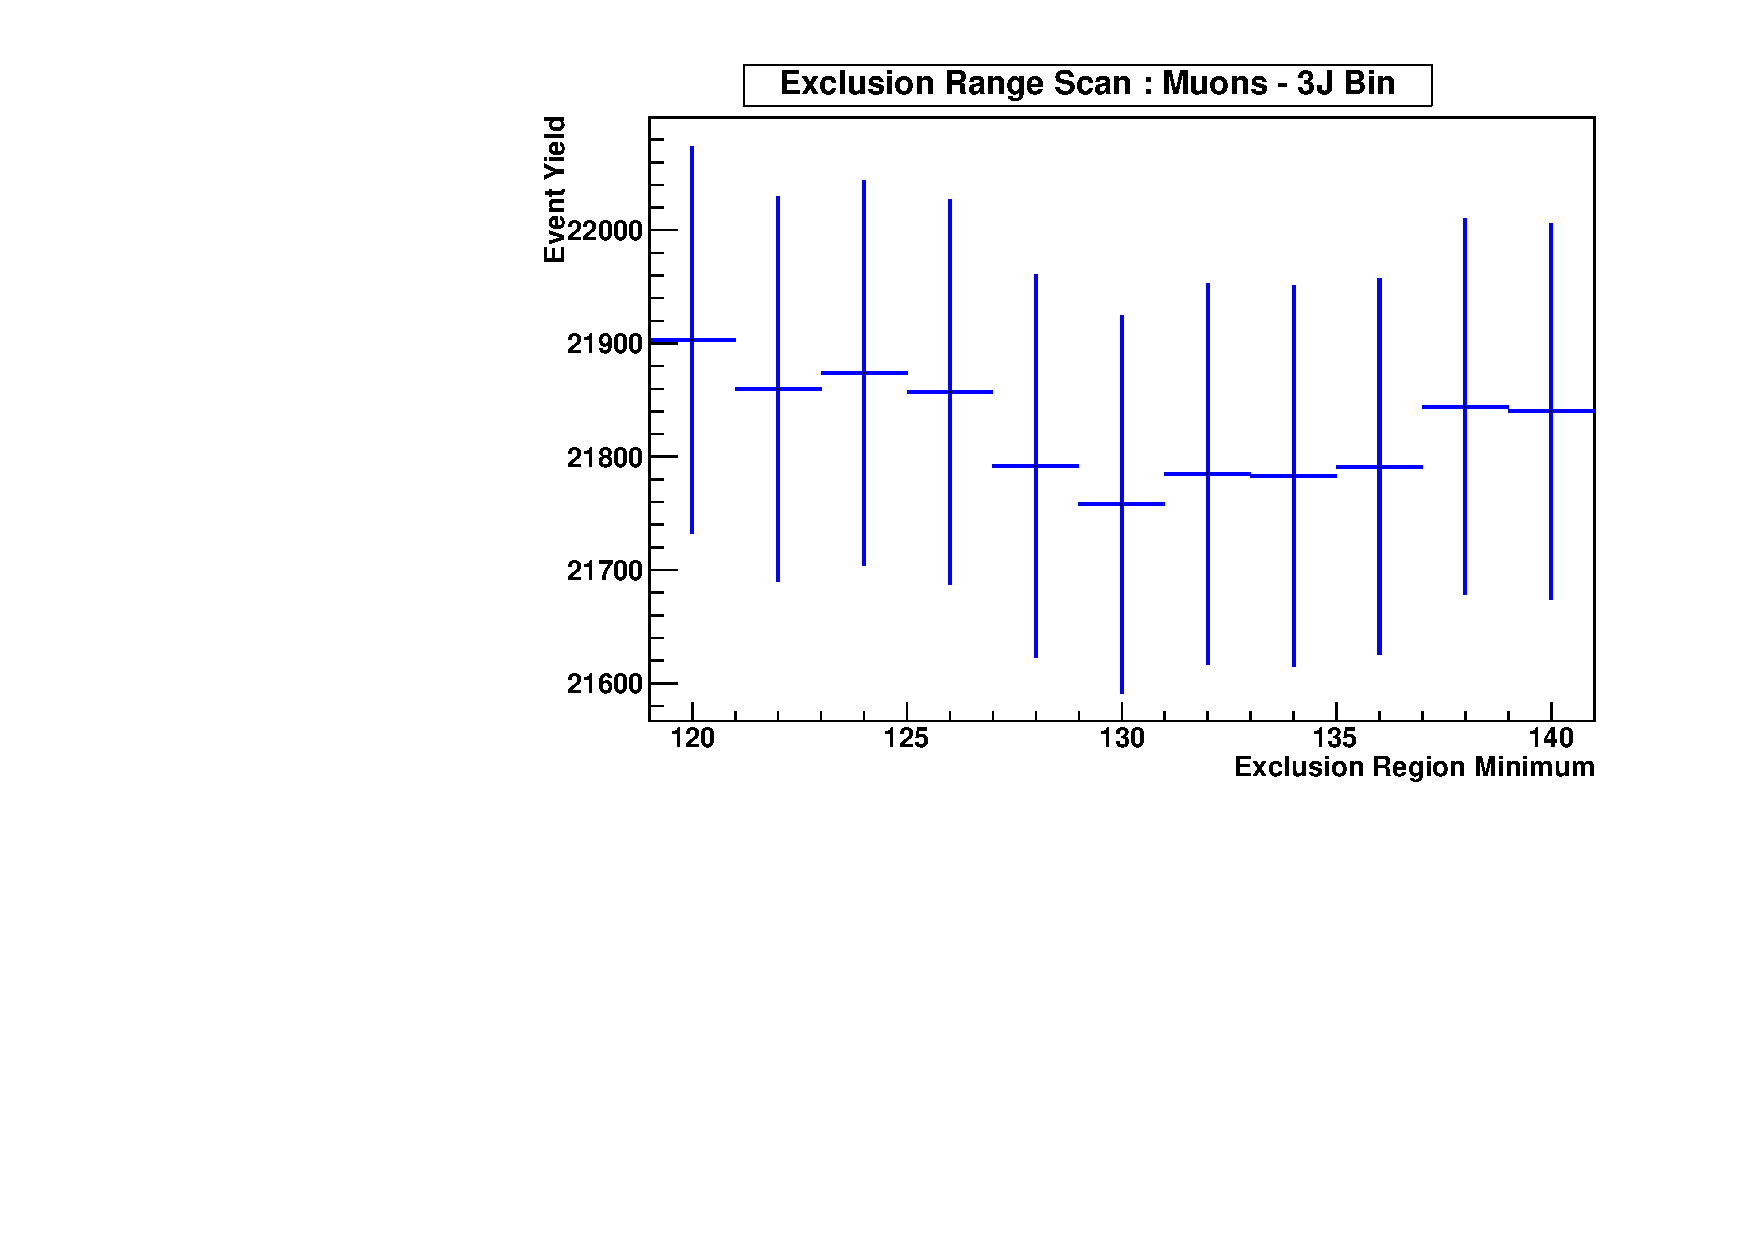
\includegraphics[width=0.48\textwidth]{figs/AdditionalStudies/ExclusionRangeScan_mu3J.pdf}
\put(-0.80,0.0){(b)} \\
\unitlength=0.33\linewidth
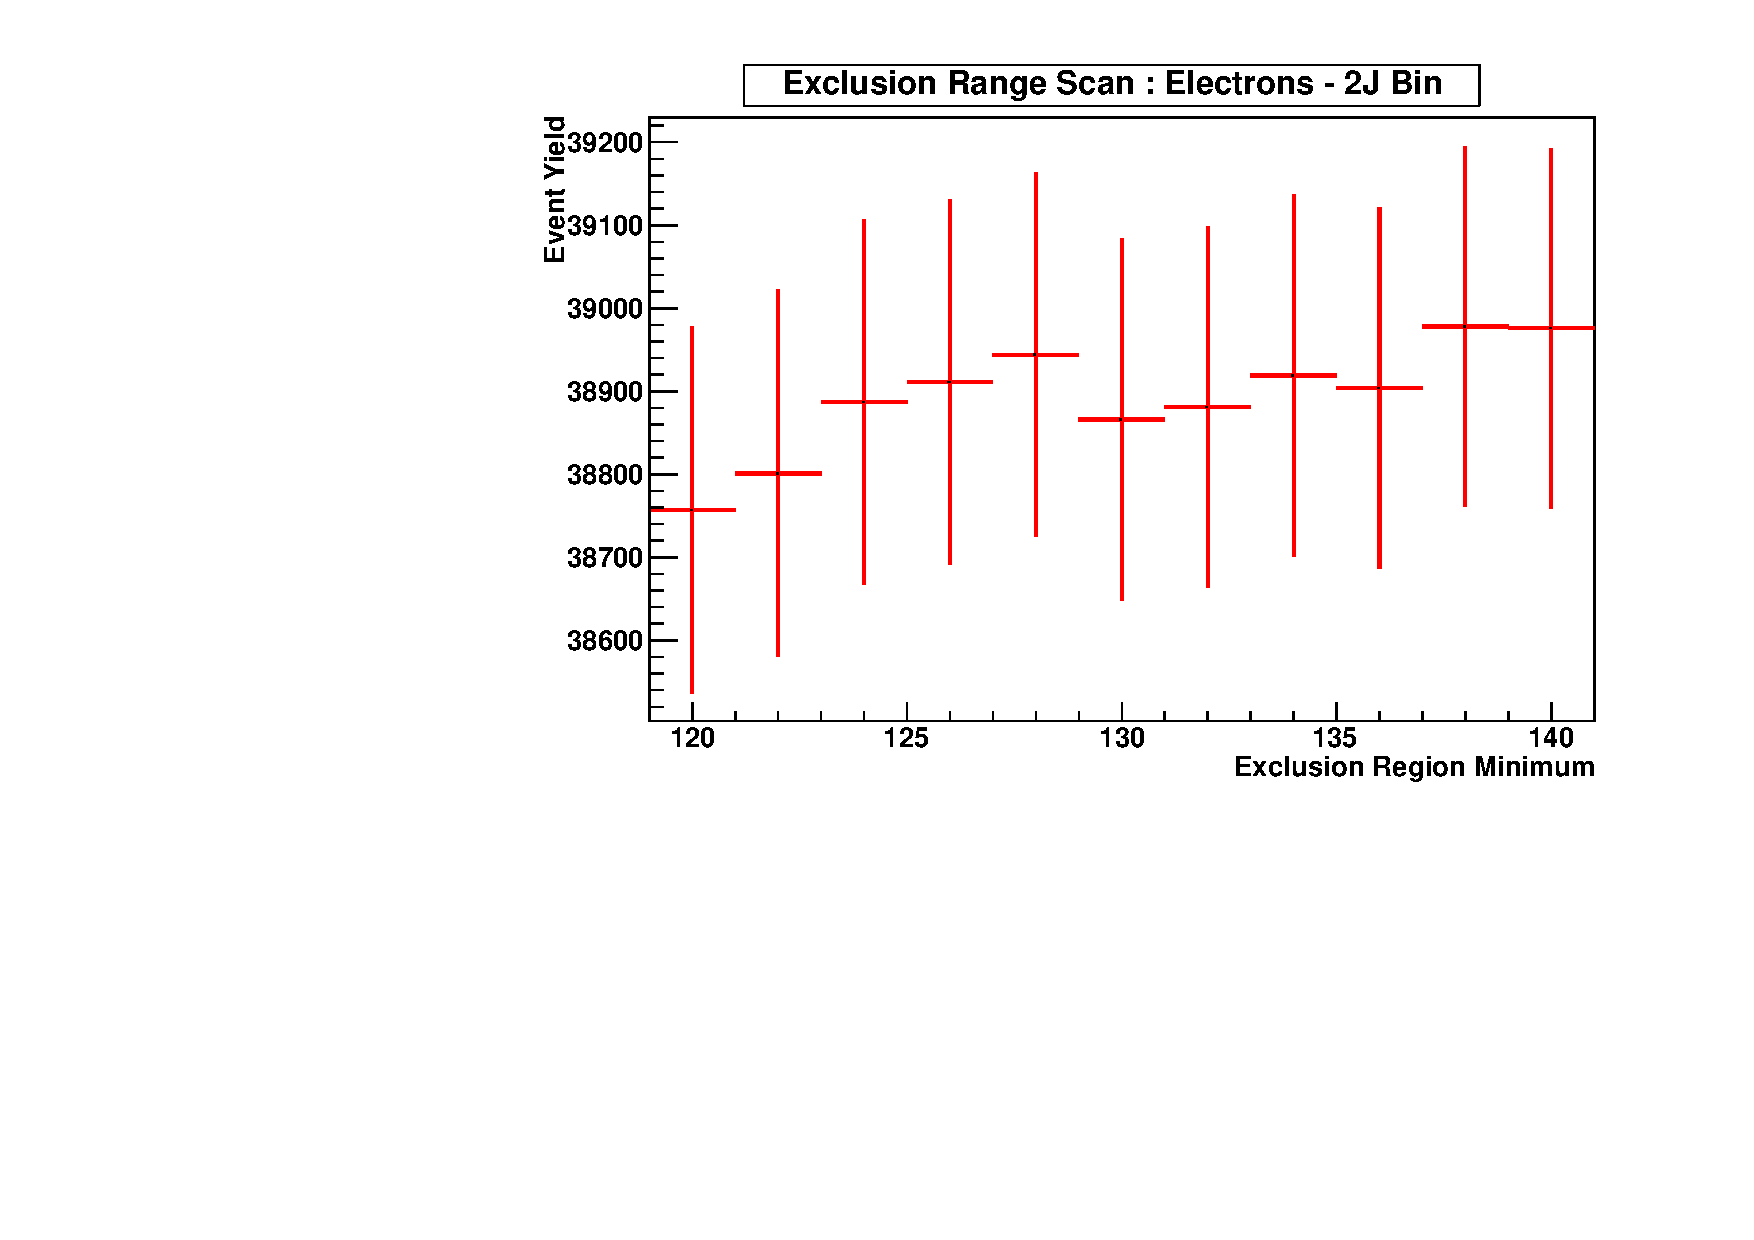
\includegraphics[width=0.48\textwidth]{figs/AdditionalStudies/ExclusionRangeScan_el2J.pdf}
\put(-0.80,0.0){(c)} 
\unitlength=0.33\linewidth
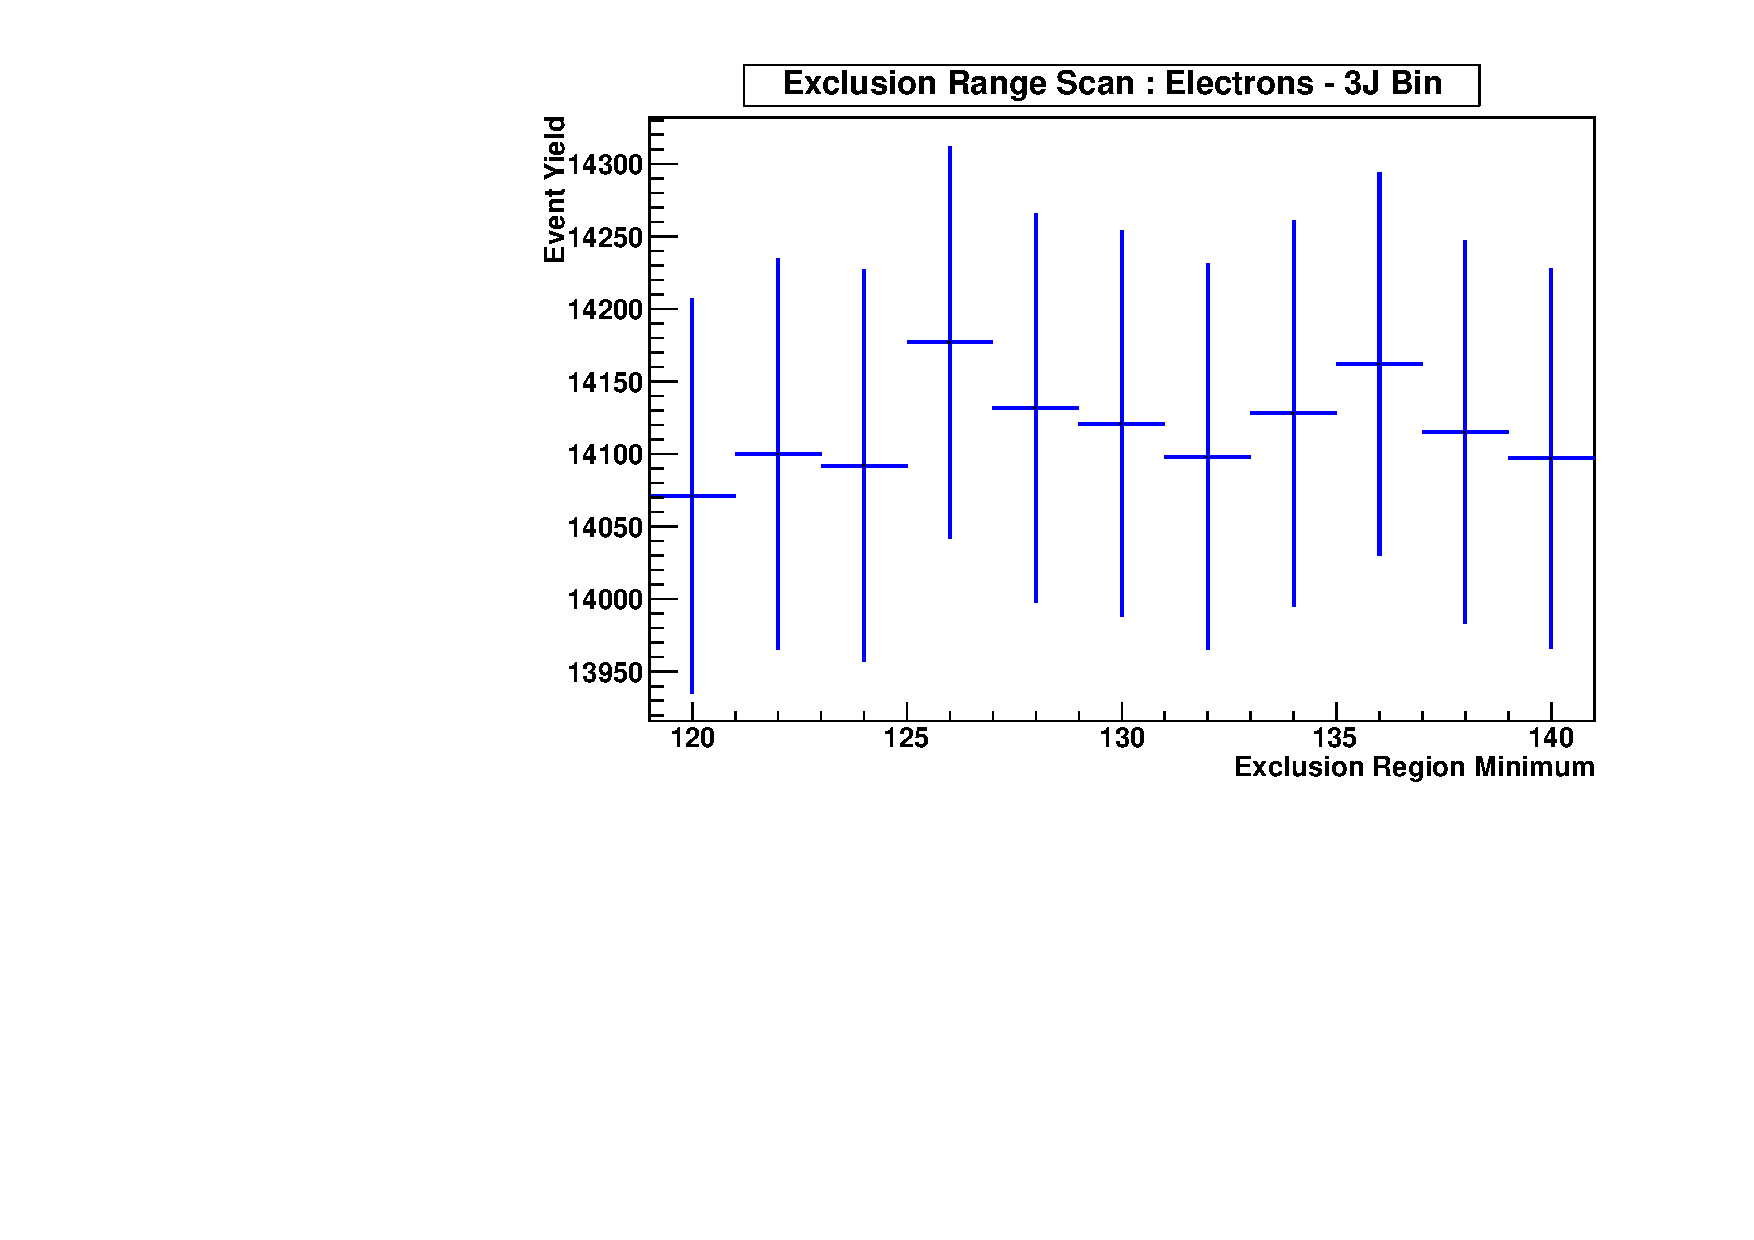
\includegraphics[width=0.48\textwidth]{figs/AdditionalStudies/ExclusionRangeScan_el3J.pdf}
\put(-0.80,0.0){(d)} 
\caption{Total Yield as a function of the lower boundary of the exlusion window (with the 
width of $42~{\mbox{GeV}}$) for : (a) muons - 2-jet bin, (b) muons - 3-jet bin, (c) electrons - 2-jet bin, (d) electrons - 3-jet bin.} 
\label{fig:ExclusionRangeScan}
}
\end{figure}
%%%%%%%
